\documentclass[11pt,a4paper]{article}
\usepackage[utf8]{inputenc}
\usepackage[T1]{fontenc}
\usepackage{lmodern}
\usepackage[margin=2.5cm]{geometry}
\usepackage{amsmath,amssymb}
\usepackage{booktabs}
\usepackage{graphicx}
\usepackage{hyperref}
\usepackage{xurl}
\usepackage{setspace}
\onehalfspacing

\hypersetup{
    colorlinks=true,
    linkcolor=blue,
    citecolor=blue,
    urlcolor=blue
}

\title{\textbf{Invisible Bridges of Credit: Exchange Rate Integration, Paper Assignats, and Metallic Anchors between St.~Petersburg and Europe, 1763--1913}}

\author{
    Petr Avtonomov\thanks{Independent Researcher, St. Petersburg, Russia. ORCID: \href{https://orcid.org}{0009-0003-2816-6782}. Code and data available at: \url{https://github.com/avtonomov-petr/Invisible-Bridges-of-Credit}}
}

\date{\today}



\begin{document}

\maketitle

\begin{abstract}
In two companion studies of grain price chronicles (\href{https://doi.org}{Avtonomov, 2026a}) and Sound Toll shipping passages (\href{https://doi.org}{Avtonomov, 2026b}), we demonstrated that before 1850 European commodity integration operated episodically around a Baltic--North Sea maritime belt and was repeatedly interrupted by winter ice and wartime blockades. Yet bills of exchange moved along postal routes even when sailing vessels stood icebound. Using the Clio Infra \emph{Exchange Rates to UK Pound} series (\texttt{1763--1913}, $T = 151$ years) paired with statutory silver and gold coinage benchmarks for the Russian ruble and British pound sterling, this paper audits the financial integration between St.~Petersburg and eight European economies. Comparing market exchange rates against statutory metallic parities reveals how paper \emph{assignats} (introduced in 1769) and Napoleonic war finance drove the St.~Petersburg ruble to 4.02 times its silver parity by 1825 (23.39 vs.\ 5.81 rubles per pound), until Count Kankrin's 1839 monetary reform restored metallic parity (6.08 rubles per pound, $1.05\times$). After late-nineteenth-century global silver depreciation shifted the pound's market silver equivalent to 13.92 rubles, Count Witte's 1897 gold standard anchored the ruble tightly at its statutory gold parity of 9.46 rubles per pound ($0.99\text{--}1.00\times$). Spectral decomposition across all nine currencies (\texttt{1764--1913}) isolates Russia as a distinct fiscal-outlier pole on Mode~2 ($v_{2,\mathrm{Russia}} = +0.503$; $\mathrm{Var}_2 = 11.9\%$). Across regime sub-panels, Russia accounted for just 1.87\% of Mode~1 variance during the assignat era (\texttt{1764--1839}; $v_{2,\mathrm{Russia}} = +0.603$), surged to 14.62\% following Kankrin's stabilization (\texttt{1840--1896}), and converged to 9.15\%—near the 11.11\% uniform network benchmark—as cross-European participation peaked under the classical gold standard (\texttt{1897--1913}; $\mathrm{PR}(v_1) = 0.778$). Finally, post-Napoleonic shock localization ($\mathrm{PR}(u_1) = 0.020$, with 56.7\% of Mode~1 energy concentrated in the 1816 post-Waterloo crisis) and near-zero non-contemporaneous lagged cross-correlations ($|r| \le 0.128$, $p > 0.21$ for lags $k \neq 0$, versus modest contemporaneous $r_0 = 0.181$, $p = 0.075$) indicate that bill arbitrage operated at intra-annual postal frequencies while annual trajectories were governed by shared monetary anchors.
\end{abstract}

\noindent\textbf{Keywords:} financial history, exchange rates, Russian Empire, St.~Petersburg Exchange, paper assignats, gold standard, silver parity, cliometrics, spectral analysis.

\section{Introduction}

When winter ice sealed the Gulf of Finland and the Danish Sound, or when naval blockades halted merchant shipping between St.~Petersburg and Western Europe, did financial markets remain connected through bills of exchange? In two preceding studies of early modern market integration, we examined first the price layer using Atlantic grain chronicles (\href{https://doi.org}{Avtonomov, 2026a}) and second the physical logistics layer using 1.27 million vessel passages in the Sound Toll Registers (\href{https://doi.org}{Avtonomov, 2026b}). Those audits established that while physical port specialization between Russia and Britain solidified immediately after 1722, commodity price arbitrage remained episodic before 1850 and was repeatedly disrupted by wartime chokepoint closures.

Bills of exchange drawn on the St.~Petersburg Exchange against Amsterdam, London, and Hamburg operated on a faster, lighter infrastructure than bulk cargo vessels, traveling along overland postal routes through Riga, Konigsberg, and Berlin throughout the winter months (Sperling, 1962; Denzel, 2010). Classic scholarship on international monetary history (Flandreau, 2004; Obstfeld \& Taylor, 2004; Officer, 1996) emphasizes how metallic convertibility and the classical gold standard bound national currencies within tight specie-point bands, whereas Russian monetary historiography (Kaufman, 1909; Crisp, 1976; Drummond, 1976; Mironov, 2010) highlights the recurring tension between domestic fiscal deficits, paper \emph{assignat} issuance after 1769, and periodic stabilization reforms under Count Egor Kankrin (1839--1843) and Count Sergei Witte (1897).

This paper serves as the capstone of our three-layer empirical audit by analyzing continuous annual exchange rate series for St.~Petersburg and eight European economies over 1763--1913 ($T = 151$ years). Combining market exchange rates against the British pound sterling with exact metallic parity benchmarks derived from pure silver and gold coinage standards, we test how the timeline of financial integration compared against physical cargo flows and commodity price arbitrage.

We establish three empirical findings:
\begin{enumerate}
    \item \textbf{Departure from and Return to Metallic Anchors:} Comparing market ruble--sterling exchange rates against statutory silver and gold parities quantifies Russia's century-long monetary cycle. Following the introduction of paper \emph{assignats} in 1769 and Napoleonic war finance, the market exchange rate diverged from its 18.00-gram silver parity (5.81--6.19 rubles per pound) to a trough of 23.39 rubles per pound in 1825 ($4.02\times$ parity). Kankrin's 1839 devaluation and silver conversion abruptly restored the metallic anchor (6.08 rubles per pound, $1.05\times$). After 1873, global silver depreciation pushed the pound's market silver equivalent to 13.92 rubles, while Witte's 1897 gold reform locked the credit ruble precisely onto its statutory gold parity of 9.46 rubles per pound ($0.99\text{--}1.00\times$).
    \item \textbf{Staged Integration into the European Monetary Core:} Across the full 1764--1913 panel ($N=9$), orthogonal Mode~2 ($\mathrm{Var}_2 = 11.9\%$) isolates Russia as a distinct fiscal-outlier pole ($v_{2,\mathrm{Russia}} = +0.503$). Evaluating fixed-composition ($N=9$) regime sub-panels shows that during the assignat and Napoleonic era (1764--1839), Russia stood outside the Western European financial core, contributing only 1.87\% to Mode~1 variance ($v_{2,\mathrm{Russia}} = +0.603$). After Kankrin's reform (1840--1896), Russia's Mode~1 variance share surged 7.8-fold to 14.62\%, and under the classical gold standard (1897--1913) network-wide spatial participation reached its historical peak ($\mathrm{PR}(v_1) = 0.778$), with Russia's share (9.15\%) converging symmetrically toward the $1/9 = 11.11\%$ uniform network benchmark.
    \item \textbf{Crisis Localization and Frequency of Bill Arbitrage:} Across the strictly uninterpolated post-Napoleonic panel (1816--1913, $M = 98$ transitions across eight countries), Mode~1 captures 30.7\% of total variance but is sharply localized in time ($\mathrm{PR}(u_1) = 0.020$), with 56.7\% of its energy concentrated in the 1816 post-Waterloo financial crisis and monetary reorganization. Non-contemporaneous annual lead--lag cross-correlations between St.~Petersburg and Amsterdam, Hamburg/Berlin, and Paris at lags $k \in \{-2, -1, +1, +2\}$ years are statistically indistinguishable from zero ($|r| \le 0.128$, $p > 0.21$), demonstrating that postal bill arbitrage operated at intra-annual (3--4 week) frequencies rather than multi-year horizons.
\end{enumerate}

\section{Data Architecture and Metallic Parity Calibration}

\subsection{Historical Exchange Rate Corpus (1763--1913)}
Primary exchange rate series are drawn from the Clio Infra \emph{Exchange Rates to UK Pound (1500--2013)} dataset (compiled from Denzel, 2010; van Zanden et al., 2014), which expresses national currency units per British pound sterling (£) on a consistent annual basis. Screening all European countries over 1700--1913 identifies 1763 as the exact starting year from which St.~Petersburg exchange quotations form an unbroken, zero-missing annual series through 1913 ($T = 151$ consecutive observations; prior to 1763, Russian quotations exhibit 41 missing years between 1722 and 1762).

To benchmark St.~Petersburg against the wider European financial network over 1763--1913, we assemble a nine-country panel ($N=9$) comprising \texttt{Russia} alongside the Western financial core (\texttt{Netherlands}, \texttt{Germany}, \texttt{France}), Northern neighbors (\texttt{Sweden}), Central Europe (\texttt{Austria}), and the Southern European periphery (\texttt{Spain}, \texttt{Portugal}, \texttt{Italy}). Within this 151-year window, \texttt{Russia}, \texttt{Germany}, \texttt{Portugal}, and \texttt{Italy} have zero missing observations, while \texttt{Netherlands} (1796--1799), \texttt{France} (1794--1795, 1798--1800), \texttt{Spain} (1798--1800), \texttt{Sweden} (1769, 1796, 1811, 1825), and \texttt{Austria} (1763, 1799, 1808--1812, 1814) exhibit minor wartime gaps during the French Revolutionary and Napoleonic conflicts. To guarantee complete methodological transparency, we evaluate both the full 1764--1913 transition panel ($M = 150$, $N=9$, bridged via linear interpolation in levels across isolated wartime gaps) and a strictly uninterpolated, zero-missing post-Napoleonic sub-panel spanning 1816--1913 ($M = 98$ transitions across the $N=8$ countries with zero missing values after 1815: \texttt{Russia}, \texttt{Netherlands}, \texttt{Germany}, \texttt{France}, \texttt{Austria}, \texttt{Spain}, \texttt{Portugal}, and \texttt{Italy}, excluding \texttt{Sweden} due to its single 1825 gap).
\subsection{Statutory Silver and Gold Parity Benchmarks}
To separate domestic paper-money inflation from international bullion movements, we calibrate exact metallic parities between the Russian ruble and the British pound using two historical bullion series from the Global Price and Income History Group (GPIHG):
\begin{itemize}
\item \textbf{Russian Coinage Standards (Mironov, 2010; GPIHG \emph{Russia Ag content ruble 1535--1913}, Table~1):} Following Empress Catherine~II's monetary decree of 1764, the statutory fine silver content of one silver ruble was fixed at exactly $Ag_{\mathrm{RUB}} = 18.00\text{ g}$ (down from $20.74\text{ g}$ in 1763) and remained unchanged through 1914. Under Count Witte's gold standard reform of 1897, the statutory fine gold content of one gold ruble was fixed at $Au_{\mathrm{RUB}} = 0.77423\text{ g}$.
\item \textbf{British Coinage and Bullion Benchmarks (Jastram, 1981, pp.~164--188; Lindert, 2006, GPIHG \emph{Silver value of £ 1273--1977}):} The statutory mint silver content of one pound sterling stood at $111.38\text{ g}$ through 1815 and $104.62\text{ g}$ following Britain's Coinage Act of 1816, yielding a statutory silver mint parity of $P^{\mathrm{Ag}}t = Ag{\mathrm{GBP},t} / Ag_{\mathrm{RUB},t} = 6.188\text{ rubles/£}$ (1764--1815) and $5.812\text{ rubles/£}$ (1816--1913). Alongside mint parity, we compute the London market silver equivalent using annual market silver prices in London, as well as the statutory gold parity after 1897 based on the British gold sovereign ($7.32238\text{ g}$ fine gold), giving $P^{\mathrm{Au}} = 7.32238 / 0.77423 = 9.458\text{ rubles/£}$.
\end{itemize}
\section{Empirical Results}
\subsection{Metallic Anchors versus Paper Assignat Depreciation}
Tracking the ratio of the St.~Petersburg market exchange rate to its active statutory metallic parity ($E^{\mathrm{mkt}}_t / P^{\mathrm{met}}_t$) across 1763--1913 illuminates four distinct monetary epochs in Imperial Russia (Figure~\ref{fig:fig1}A and Figure~\ref{fig:fig2}B).
\begin{figure}[htbp]
\centering
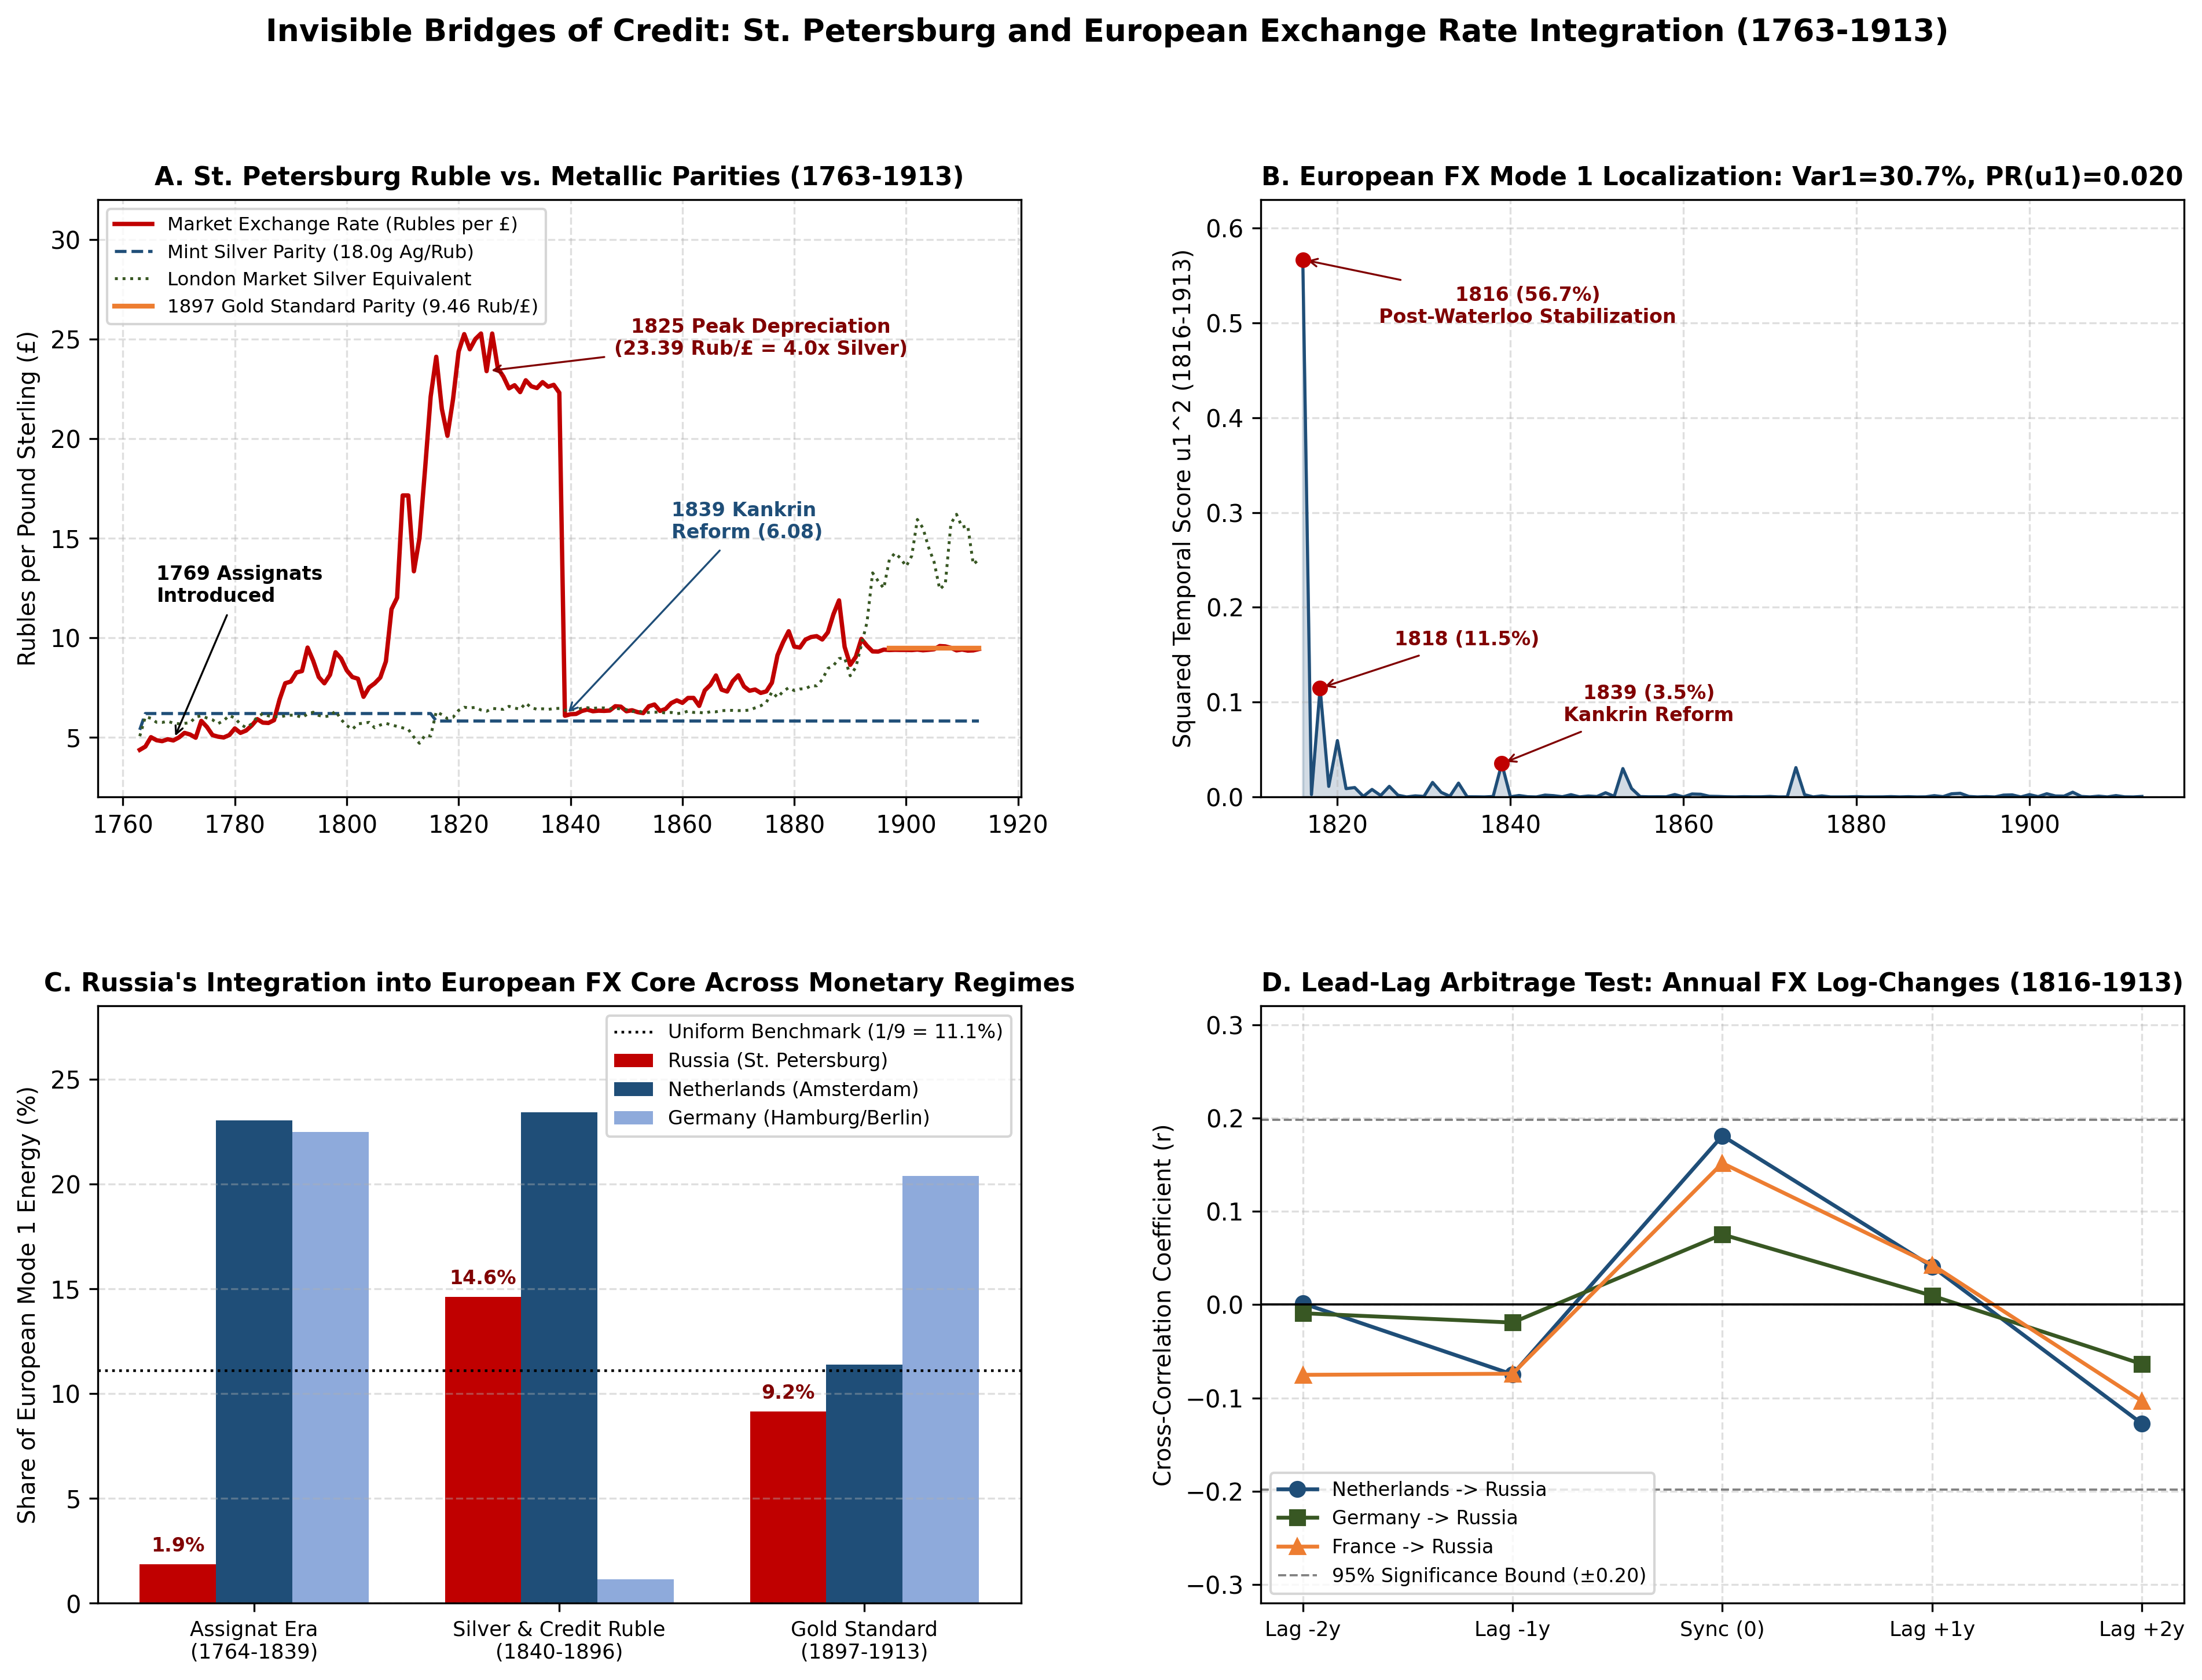
\includegraphics[width=\textwidth]{Figure_1_FX.png}
\caption{\textbf{St.~Petersburg Exchange Rate Integration and Metallic Parities (1763--1913).} \textbf{A:} Market exchange rate (rubles per \pounds) compared against statutory silver mint parity, London market silver equivalent, and the 1897 gold standard parity. \textbf{B:} Temporal localization of European Mode~1 energy ($u_{t,1}^2$, 1816--1913), highlighting the 1816 post-Waterloo financial crisis and monetary reorganization (56.7\%). \textbf{C:} Russia's share of European Mode~1 variance across three fixed-composition ($N=9$) monetary regimes relative to Amsterdam and Germany. \textbf{D:} Annual lead--lag cross-correlations between Western financial hubs and St.~Petersburg (1816--1913).}
\label{fig:fig1}
\end{figure}

Prior to 1769, Russian bills traded near or slightly below silver parity ($0.78\text{--}0.81\times$, reflecting Russia's persistent Baltic trade surplus). Following the introduction of paper \emph{assignats} in 1769 to finance the Russo-Turkish War, unbacked paper issuance gradually eroded the ruble's external value to $1.12\times$ parity by 1788 and $1.35\times$ by 1800. During the Napoleonic Wars and Continental Blockade, massive fiscal deficits drove the exchange rate to 17.14 rubles per pound in 1810 ($2.77\times$ silver parity), 18.46 in 1814 ($2.98\times$), and an all-time trough of 23.39 rubles per pound in 1825 ($4.02\times$ silver parity).
Count Kankrin's monetary stabilization of 1839—which fixed the conversion rate at 3.50 paper assignat rubles per silver ruble—abruptly snapped the exchange rate back to 6.08 rubles per pound ($1.05\times$ statutory silver parity). Convertibility survived until the Crimean War (1854--1856, $1.14\times$) and the Russo-Turkish War of 1877--1878, when renewed credit-ruble issuance pushed the rate to 9.77 rubles per pound ($1.68\times$ mint silver parity). Crucially, however, after 1873 the global demonetization of silver caused the London market silver equivalent of the gold pound to climb toward 13.92 rubles per pound (Figure~\ref{fig:fig1}A). Rather than following depreciating silver downward, the Russian credit ruble stabilized around $9.38\text{--}9.43$ rubles per pound, allowing Count Witte's 1897 gold standard to lock the currency seamlessly onto its statutory gold parity of 9.458 rubles per pound ($0.99\text{--}1.00\times$ through 1913).
\subsection{Network Decomposition Across European Monetary Regimes}
Applying singular value decomposition and participation ratio diagnostics (Appendix~A) to annual log-changes $\Delta \ln E_{t,j}$ across the nine-currency panel reveals how Russia's structural position evolved across monetary regimes (Table~\ref{tab:fx_summary} and Figure~\ref{fig:fig2}A).

\begin{table}[htbp]
\centering
\caption{Spectral and Topological Summary of European Exchange Rate Integration (1764--1913)}
\label{tab:fx_summary}
\footnotesize
\setlength{\tabcolsep}{4.2pt}
\begin{tabular}{lccccc}
\toprule
\textbf{Sample / Monetary Regime} & \textbf{Trans. ($M$)} & \textbf{Mode 1 Var.} & \textbf{Temporal $\mathrm{PR}(u_1)$} & \textbf{Spatial $\mathrm{PR}(v_1)$} & \textbf{Russia Share} \tabularnewline
\midrule
Full European Panel (1764--1913, $N=9$) & 150 & 25.7\% & 0.095 [0.075, 0.128] & 0.558 [0.464, 0.719] & 4.32\% \tabularnewline
Uninterpolated Clean (1816--1913, $N=8$) & 98 & 30.7\% & 0.020 [0.012, 0.084] & 0.428 [0.372, 0.688] & 3.94\% \tabularnewline
Assignat and Napoleonic Era (1764--1839, $N=9$) & 76 & 35.5\% & 0.158 [0.119, 0.220] & 0.610 [0.557, 0.744] & 1.87\% \tabularnewline
Silver and Credit Ruble Era (1840--1896, $N=9$) & 57 & 19.9\% & 0.205 [0.114, 0.278] & 0.711 [0.327, 0.764] & 14.62\% \tabularnewline
Classical Gold Standard (1897--1913, $N=9$) & 17 & 35.2\% & 0.346 [0.226, 0.453] & 0.778 [0.523, 0.847] & 9.15\% \tabularnewline
\bottomrule
\end{tabular}
\vspace{1mm}
\begin{minipage}{\textwidth}
\footnotesize\emph{Notes:} Diagnostics computed on standardized annual log-changes $\Delta \ln E_{t,j}$ of exchange rates against the British pound sterling. Uniform cross-sectional energy benchmark is $1/9 = 11.11\%$ for $N=9$ and $1/8 = 12.50\%$ for $N=8$. Brackets report 95\% subsampling bootstrap confidence intervals (300 draws at 80\% sample length).
\end{minipage}
\end{table}

Over the full 1764--1913 sample ($M = 150$, $N=9$), Mode~1 accounts for 25.7\% of total variance and is anchored by the Western European financial core: \texttt{Netherlands} (29.37\% of Mode~1 energy), \texttt{Germany} (21.24\%), and \texttt{France} (15.17\%). In contrast, \texttt{Russia} accounts for only 4.32\% of Mode~1 variance, and orthogonal Mode~2 ($\mathrm{Var}_2 = 11.9\%$; Figure~\ref{fig:fig2}A) isolates Russia at the extreme positive pole ($v_{2,\mathrm{Russia}} = +0.503$) opposite the Southern European periphery (\texttt{Spain} $-0.615$, \texttt{Italy} $-0.481$) and the Western core (\texttt{Germany} $-0.173$, \texttt{France} $-0.050$, \texttt{Netherlands} $-0.029$).

Sub-period decomposition on the identical nine-country roster ($N=9$) demonstrates that Russia's financial integration proceeded in three distinct stages (Figure~\ref{fig:fig1}C):
\begin{itemize}
    \item \textbf{Assignat Isolation (1764--1839, $M=76$, $N=9$):} While Western Europe experienced synchronized Napoleonic war and stabilization swings ($\mathrm{Var}_1 = 35.5\%$), Russia's domestic paper-money depreciation decoupled St.~Petersburg from Europe, leaving Russia with just 1.87\% of Mode~1 energy and an isolated Mode~2 loading of $v_{2,\mathrm{Russia}} = +0.603$ ($\mathrm{Var}_2 = 12.1\%$).
    \item \textbf{Post-Kankrin Reintegration (1840--1896, $M=57$, $N=9$):} Following the 1839 return to silver, Russia's share of Mode~1 energy jumped 7.8-fold to 14.62\% (ranking third behind \texttt{Netherlands} at 23.44\% and \texttt{Spain} at 16.54\%), with shared European fluctuations driven by the 1847 financial crisis (12.8\% of Mode~1 energy) and the Crimean War of 1853--1854 (27.0\% combined).
    \item \textbf{Gold Standard Convergence (1897--1913, $M=17$, $N=9$):} Under the international gold standard, network-wide spatial participation expanded to its historical peak ($\mathrm{PR}(v_1) = 0.778$, $\mathrm{Var}_1 = 35.2\%$) while temporal shock concentration fell to its lowest level ($\mathrm{PR}(u_1) = 0.346$). Rather than reflecting outlier dominance as in the 1850s, Russia's 9.15\% variance share aligned closely with the $1/9 = 11.11\%$ uniform network benchmark alongside \texttt{Germany} (20.40\%), \texttt{Sweden} (17.30\%), \texttt{Italy} (14.95\%), and \texttt{Netherlands} (11.40\%) during the global liquidity crises of 1899 and 1907--1908.
\end{itemize}

\begin{figure}[htbp]
\centering
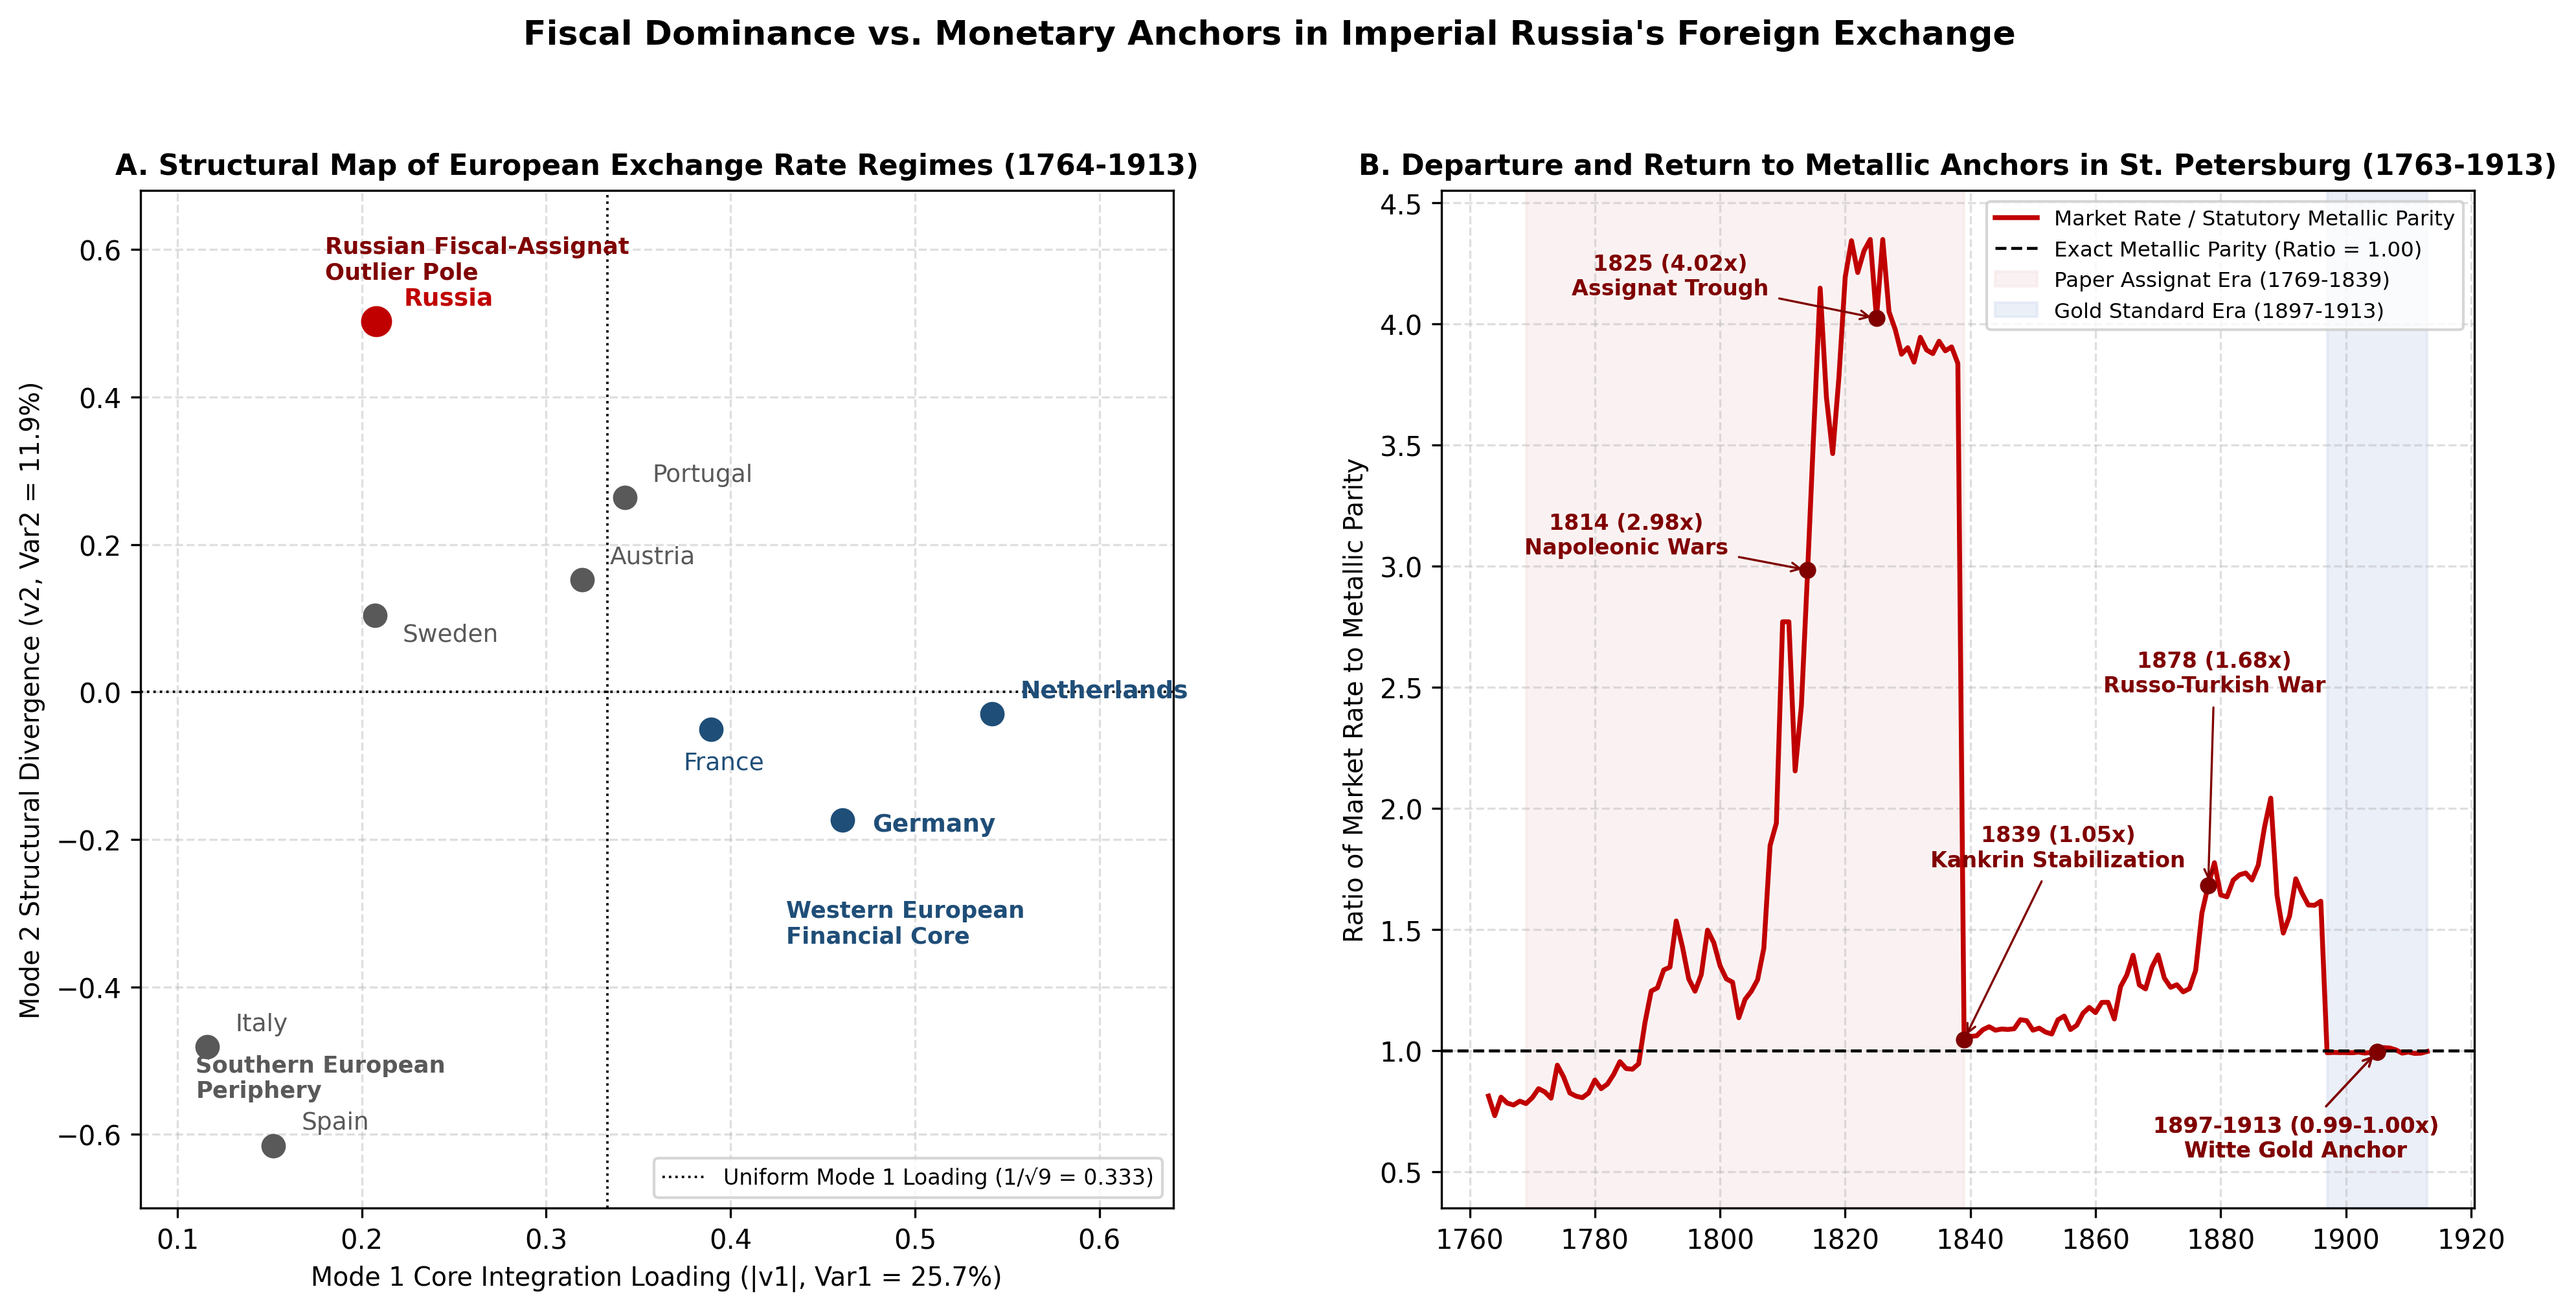
\includegraphics[width=\textwidth]{Figure_2_FX.png}
\caption{\textbf{Fiscal Dominance versus Monetary Anchors in Imperial Russia's Foreign Exchange.} \textbf{A:} Two-mode structural map of European currencies (1764--1913), contrasting the Western European financial core against Russia's fiscal-assignat pole and Southern European silver periphery. \textbf{B:} Ratio of the St.~Petersburg market exchange rate to its active statutory metallic parity (1763--1913), tracing the fourfold assignat depreciation peak in 1825, Kankrin's 1839 stabilization, wartime credit-ruble departures, and Witte's 1897 gold anchor.}
\label{fig:fig2}
\end{figure}

\subsection{Shock Localization and the Frequency of Bill Arbitrage}
Evaluating the strictly uninterpolated post-Napoleonic panel (1816--1913, $M = 98$, $N = 8$) confirms that annual exchange rate synchronization was overwhelmingly shock-driven rather than continuous (Figure~\ref{fig:fig1}B). Although Mode~1 captures 30.7\% of total variance, its temporal participation ratio is $\mathrm{PR}(u_1) = 0.020$ ($[0.012, 0.084]$), with 56.7\% of all Mode~1 temporal energy concentrated in the single transition of 1816 (the post-Waterloo financial crisis and monetary reorganization across Amsterdam, Paris, and London) and another 11.5\% in 1818. Consistently, the transition graph scan detects no abrupt structural break inside the nineteenth century ($p = 0.069$ for 1764--1913; $p = 0.105$ for 1816--1913), indicating gradual institutional convergence rather than a single overnight regime switch.

Finally, computing annual lead--lag cross-correlations between Western European financial hubs (\texttt{Netherlands}, \texttt{Germany}, \texttt{France}) and \texttt{Russia} across lags $k \in \{-2, -1, 0, +1, +2\}$ years over 1816--1913 illuminates the operating frequency of foreign exchange arbitrage (Figure~\ref{fig:fig1}D). Contemporaneous annual co-movement is modest ($r_0 = 0.181$, $p = 0.075$ with \texttt{Netherlands}; $r_0 = 0.152$, $p = 0.136$ with \texttt{France}; $r_0 = 0.075$, $p = 0.462$ with \texttt{Germany}), while all non-contemporaneous lagged correlations ($k \neq 0$) lie well inside the 95\% white-noise significance bounds ($\pm 0.20$): for Amsterdam $\to$ St.~Petersburg, $r_{-1} = -0.075$ ($p = 0.466$) and $r_{+1} = 0.041$ ($p = 0.692$); for Germany $\to$ St.~Petersburg, $r_{-1} = -0.019$ ($p = 0.852$) and $r_{+1} = 0.010$ ($p = 0.926$); and for Paris $\to$ St.~Petersburg, $r_{-1} = -0.074$ ($p = 0.471$) and $r_{+1} = 0.043$ ($p = 0.678$). Historically, postal transmission between Amsterdam, Hamburg, and St.~Petersburg required three to four weeks rather than one to two years. Consequently, the absence of multi-year lagged predictability proves that bill arbitrage cleared on intra-annual (weekly to monthly) horizons within metallic specie points, leaving annual exchange rate variations to reflect domestic fiscal regimes and shared international monetary anchors.

\section{Discussion: Three Asynchronous Layers of Integration}

Synthesizing this currency audit with our preceding studies of grain price chronicles (\href{https://doi.org}{Avtonomov, 2026a}) and Sound Toll shipping passages (\href{https://doi.org}{Avtonomov, 2026b}) reveals that Russian--European economic integration did not unfold as a single synchronized wave, but progressed sequentially across three functional layers separated by more than a century (Table~\ref{tab:three_layers}).

\begin{table}[htbp]
\centering
\caption{Three Asynchronous Layers of Russian--European Market Integration (1700--1914)}
\label{tab:three_layers}
\footnotesize
\setlength{\tabcolsep}{4pt}
\begin{tabular}{@{}p{0.23\textwidth}p{0.25\textwidth}p{0.24\textwidth}p{0.22\textwidth}@{}}
\toprule
\textbf{Integration Layer} & \textbf{Primary Archive and Metric} & \textbf{Onset of Structural Lock-In} & \textbf{Primary Bottleneck / Anchor} \tabularnewline
\midrule
1. Physical Maritime Trade & Sound Toll Registers (1700--1856) & Immediate post-1722 specialization & Naval blockades and winter ice \tabularnewline
2. Commodity Price Arbitrage & Allen--Unger Grain Series (1729--1914) & Episodic pre-1850; structural post-1850 & Interior transport and Corn Laws \tabularnewline
3. Foreign Exchange & Clio Infra FX and Bullion (1763--1913) & Post-1839 silver; 1897 gold convergence & Paper assignats and metallic parity \tabularnewline
\bottomrule
\end{tabular}
\vspace{1mm}
\begin{minipage}{\textwidth}
\footnotesize\emph{Notes:} Synthesis of findings across Avtonomov (2026a), Avtonomov (2026b), and the present study.
\end{minipage}
\end{table}


In the physical trade layer, St.~Petersburg and Riga locked into a specialized industrial-naval supply chain with Britain immediately after 1722, exporting hemp, bar iron, flax, tallow, and timber despite recurring wartime blockades. In the commodity price layer, broad food-price co-movement emerged over a century later, once interior transport improvements, steam navigation, and the repeal of the British Corn Laws allowed Russian ports to serve as elastic grain lifelines during Western subsistence crises (1817 and 1847). Finally, in the monetary and credit layer, paper \emph{assignat} issuance after 1769 detached the St.~Petersburg ruble from European metallic parities for seven decades, delaying full network convergence until Count Kankrin's 1839 silver stabilization and Count Witte's 1897 gold standard. Across all three layers, globalization emerged as a punctuated institutional achievement built sequentially on trade corridors, transport infrastructure, and credible metallic anchors.

\section*{Data and Code Availability}
All underlying historical series are openly accessible from Clio Infra (\url{https://clio-infra.eu}, \emph{Exchange Rates to UK Pound, 1500--2013}) and the Global Price and Income History Group (\url{https://ucdavis.edu}: Lindert, 2006, \emph{Silver value of \pounds{} 1273--1977}; Mironov, 2010, \emph{Russia Ag content ruble 1535--1913}). Reproducible Python/Jupyter code, high-resolution figures, and LaTeX manuscript sources are openly archived on GitHub at \url{https://github.com/avtonomov-petr/Invisible-Bridges-of-Credit}.

\appendix
\section{Mathematical Specification of Diagnostics}
Let $E_{t,j} > 0$ denote the annual exchange rate of country $j \in \{1,\dots,N\}$ expressed in national currency units per British pound sterling in year $t$. We compute annual log-changes $y_{t,j} = \ln E_{t,j} - \ln E_{t-1,j}$ over $M$ transitions and standardize each series to zero mean and unit variance, $Z_{t,j} = (y_{t,j} - \bar{y}j)/s_j$. Thin singular value decomposition $Z = U \Sigma V^\top$ yields orthonormal temporal scores $u_k \in \mathbb{R}^M$ and country loadings $v_k \in \mathbb{R}^N$. Temporal and cross-sectional localization are measured via normalized participation ratios:
\begin{equation}
\mathrm{PR}(u_1) = \frac{\left(\sum{t=1}^M u_{t,1}^4\right)^{-1} - 1}{M - 1}, \qquad
\mathrm{PR}(v_1) = \frac{\left(\sum_{j=1}^N v_{j,1}^4\right)^{-1} - 1}{N - 1}.
\end{equation}
Structural regime breaks are tested non-parametrically by constructing a symmetric $k$-nearest-neighbor Gaussian affinity graph ($k=6$, calibrated to the compact cross-sectional dimension $N=9$ compared with $k=8$ in higher-dimensional maritime networks; bandwidth $\sigma$ equal to the median pairwise Euclidean distance among rows of $Z$), extracting the Fiedler eigenvector $\psi_2$ of the normalized graph Laplacian $L_{\mathrm{sym}} = I - D^{-1/2} A D^{-1/2}$, and evaluating candidate split years $\tau \in [12, M-12]$ via two-sided Mann--Whitney $U$ tests.
\begin{thebibliography}{99}
\bibitem{Avtonomov2026a}
Avtonomov, P. (2026a). Crisis echoes or arbitrage? Selective co-movement and integration of the Atlantic grain market, 1729--1914. \emph{Zenodo Preprint}. \url{https://doi.org/10.5281/zenodo.24436177}

\bibitem{Avtonomov2026b}
Avtonomov, P. (2026b). Blockades, flag mimicry, and grain lifelines: Physical anatomy of Russian and Baltic maritime trade in the Sound Toll Registers, 1700--1856. \emph{Zenodo Preprint}. \url{https://doi.org/10.5281/zenodo.24461586}

\bibitem{Crisp1976}
Crisp, O. (1976). \emph{Studies in the Russian economy before 1914}. Macmillan.
\bibitem{Denzel2010}
Denzel, M. A. (2010). \emph{Handbook of world exchange rates, 1590--1914}. Ashgate.
\bibitem{Drummond1976}
Drummond, I. M. (1976). The Russian gold standard, 1897--1914. \emph{Journal of Economic History}, 36(3), 663--688.
\bibitem{Flandreau2004}
Flandreau, M. (2004). \emph{The glitter of gold: France, bimetallism, and the emergence of the international gold standard, 1848--1873}. Oxford University Press.
\bibitem{Jastram1981}
Jastram, R. W. (1981). \emph{Silver: The restless metal}. John Wiley \& Sons.

\bibitem{Kaufman1909}
Kaufman, I. I. (1909). \emph{Serebryanyi rubl' v Rossii ot ego vozniknoveniia do kontsa XIX veka} [The silver ruble in Russia from its origin to the end of the 19th century]. Tipografiia B. M. Vol'fa.

\bibitem{Lindert2006}
Lindert, P. H. (2006). \emph{Silver in Britain: Mint prices 1273--1971 and market prices 1693--1977}. Global Price and Income History Group, UC Davis.

\bibitem{Mironov2010}
Mironov, B. N. (2010). \emph{Blagosostoianie naseleniia i revoliutsii v imperskoi Rossii: XVIII -- nachalo XX veka} [Living standards and revolutions in Imperial Russia, 18th -- early 20th centuries]. Novyi Khronograf.

\bibitem{Obstfeld2004}
Obstfeld, M., \& Taylor, A. M. (2004). \emph{Global capital markets: Integration, crisis, and growth}. Cambridge University Press.

\bibitem{Officer1996}
Officer, L. H. (1996). \emph{Between the dollar-sterling gold points: Exchange rates, parity, and market behavior}. Cambridge University Press.

\bibitem{Sperling1962}
Sperling, J. (1962). The international payments mechanism in the seventeenth and eighteenth centuries. \emph{Economic History Review}, 14(3), 446--468.

\bibitem{vanZanden2014}
van Zanden, J. L., Baten, J., Mira d'Ercole, M., Rijpma, A., Smith, C., \& Timmer, M. (Eds.). (2014). \emph{How was life? Global well-being since 1820}. OECD Publishing.

\end{thebibliography}

\section*{Figure Alt Text}
\begin{itemize}
\item \textbf{Figure 1 Alt Text:} Four-panel chart of St.~Petersburg ruble exchange rates against silver and gold parities, European shock localization, regime shares, and lead--lag cross-correlations.
\item \textbf{Figure 2 Alt Text:} Scatter plot of nine European currency modes and time series of St.~Petersburg market exchange rate to metallic parity ratio.
\end{itemize}
\end{document}